\documentclass[12pt]{article}
\usepackage[utf8]{inputenc}
\usepackage{graphicx}
\usepackage{hyperref}
\usepackage[a4paper,width=150mm,top=25mm,bottom=25mm]{geometry}
\usepackage{float}
\usepackage[utf8]{vietnam}
\title{
{
\includegraphics[width=4.5cm, height=4.5cm]{Figs/logo-uit-300x248.png}
}
\\
{Báo Cáo Đồ Án Cuối Kì - IE303.N21.CNCL \\ Spring Movie Review}
}



\author{Hoàng Tân, Mai Anh, Quỳnh Hương \\ Giảng viên hướng dẫn: Nguyễn Văn Kiệt }

\begin{document}

\maketitle
\tableofcontents
\section{Giới thiệu đồ án}
\subsection{Tổng quan về đồ án}
Đồ án này nhằm mục đích nghiên cứu và phát triển một ứng dụng web dựa trên framework Spring Boot, được xây dựng để quản lý thông tin về phim. Ứng dụng cung cấp các tính năng cho người dùng như đề xuất, tìm kiếm, xem thông tin chi tiết, và đánh giá phim.

Mục tiêu của đồ án là tạo ra một nền tảng linh hoạt và dễ dàng mở rộng, cho phép người dùng tìm kiếm và khám phá các bộ phim dựa trên nhiều tiêu chí như thể loại, năm sản xuất, và tên phim. Đồng thời, ứng dụng cũng cung cấp tính năng đánh giá và đề xuất phim dựa trên sở thích của người dùng.

Để đạt được mục tiêu này, chúng mình sử dụng Spring Boot làm nền tảng phát triển chính, kết hợp với các công nghệ và thư viện phổ biến như PostgreSQL, Thymeleaf, Bootstrap, và Hibernate. Ứng dụng được xây dựng theo kiến trúc MVC (Model-View-Controller), giúp tách biệt logic xử lý, giao diện và dữ liệu.

Trong phần còn lại của báo cáo, chúng mình sẽ trình bày chi tiết về thiết kế và triển khai của ứng dụng, cũng như kết quả đạt được và các hướng phát triển tiềm năng.

\begin{figure}[H]
    \centering
    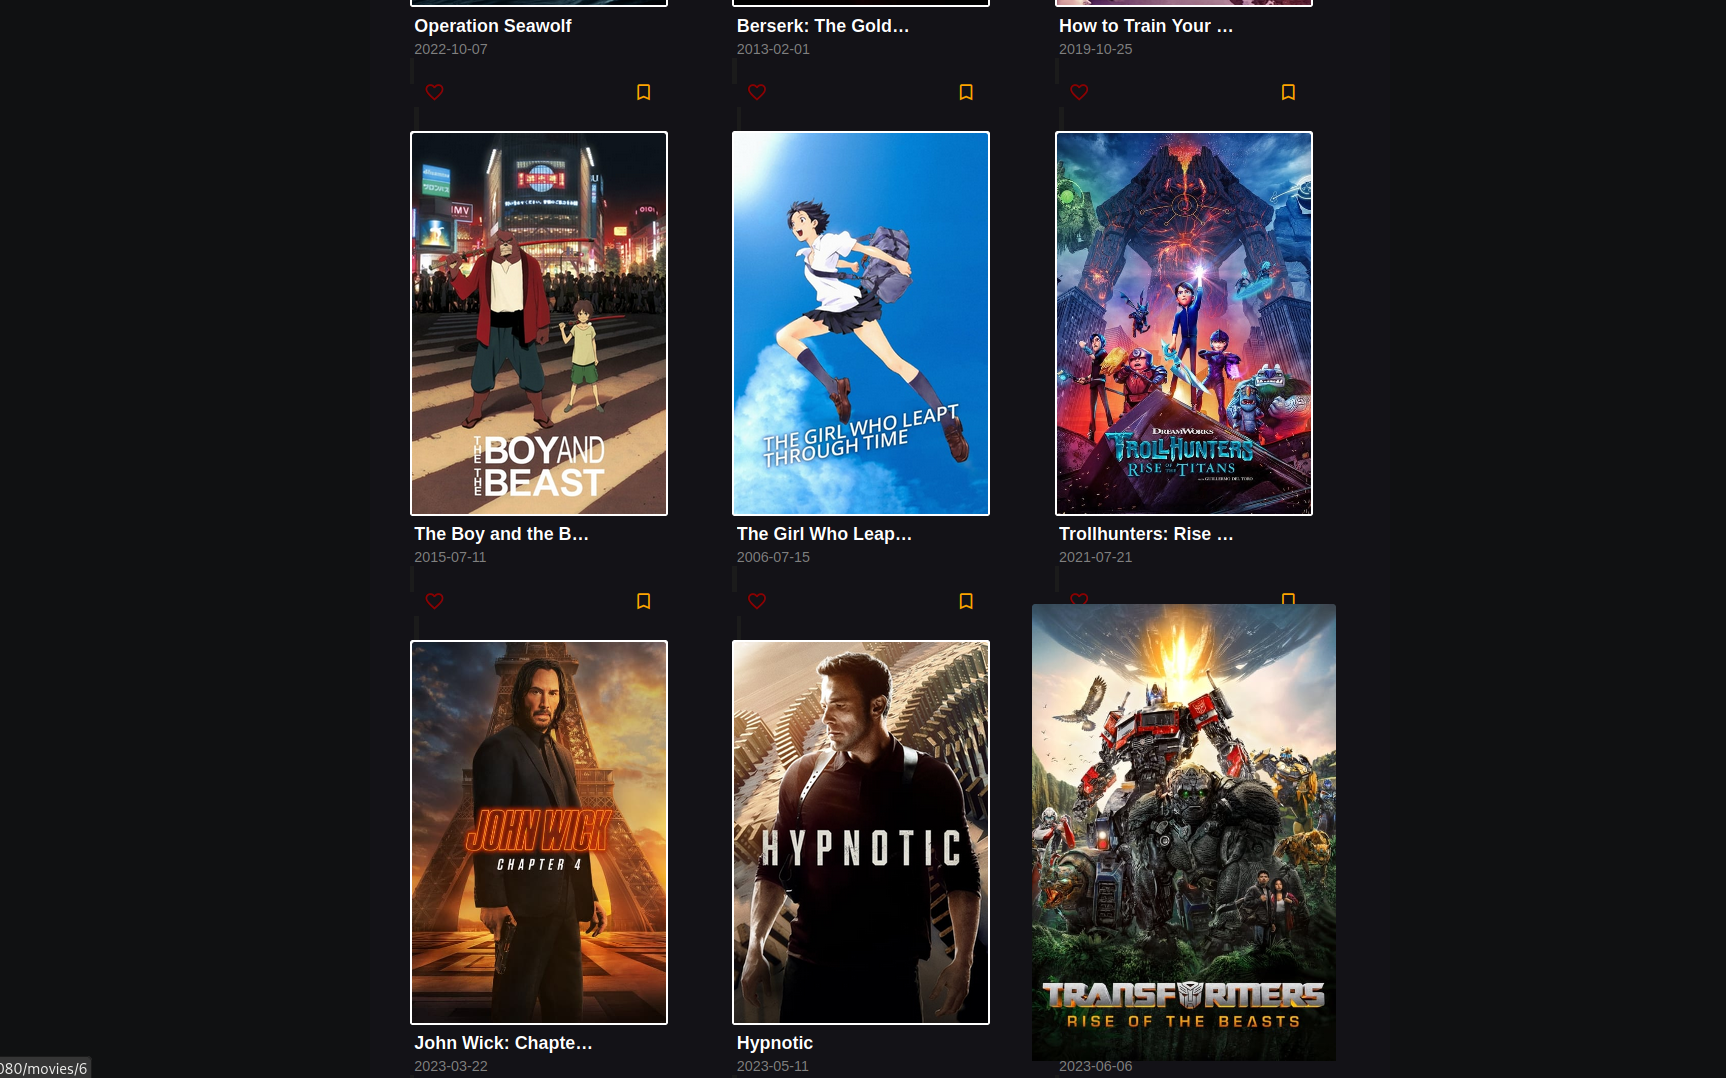
\includegraphics[scale=0.35]{Figs/Project_Review.png}
    \caption{Spring Boot Review Website}
\end{figure}
\subsection{ Đặt vấn đề}
Trong thời đại công nghệ thông tin phát triển mạnh mẽ như hiện nay, ngành công nghiệp điện ảnh đang trở thành một phần không thể thiếu của cuộc sống hàng ngày. Việc tìm kiếm và khám phá các bộ phim phù hợp với sở thích cá nhân đã trở thành một thách thức cho nhiều người.

Theo báo cáo được công bố của Akamai và Viettel IDC năm 2020, ước tính trung bình người Việt Nam trong độ tuổi từ 16 đến 64 tuổi dành 6,5 giờ mỗi ngày trên Internet, trong khi chỉ dành 2 giờ để xem TV. Đặc biệt trong nhóm người dùng Internet, 95\% người dùng sử dụng để xem các video trực tuyến, 73\% để nghe nhạc trực tuyến, 57\% để xem vlog. 
Theo khảo sát “Why video?" Ipsos 2022, thống kê cho thấy YouTube Short hiện đang thu hút tới 30 tỷ lượt xem mỗi ngày, tăng trưởng gấp 4 lần so với năm 2021 và có 1,5 tỷ người dùng đăng nhập hàng tháng. Những con số này đang tiếp tục tăng trưởng với người xem ở mọi độ tuổi, bao gồm GenZ. Theo Business of Apps, trung bình mỗi người dùng sẽ dành khoảng 52 phút mỗi ngày để sử dụng Tik Tok (bao gồm cả việc xem, tạo video hoặc chia sẻ video). Đây cũng là nền tảng một sáng tạo video ngắn rất được người dùng yêu thích. Thấy được rằng, người dùng ngày càng quan tâm đến những nền tảng truyền tải nội dung ngắn gọn, không mất nhiều thời gian.
\begin{figure}[H]
    \centering
    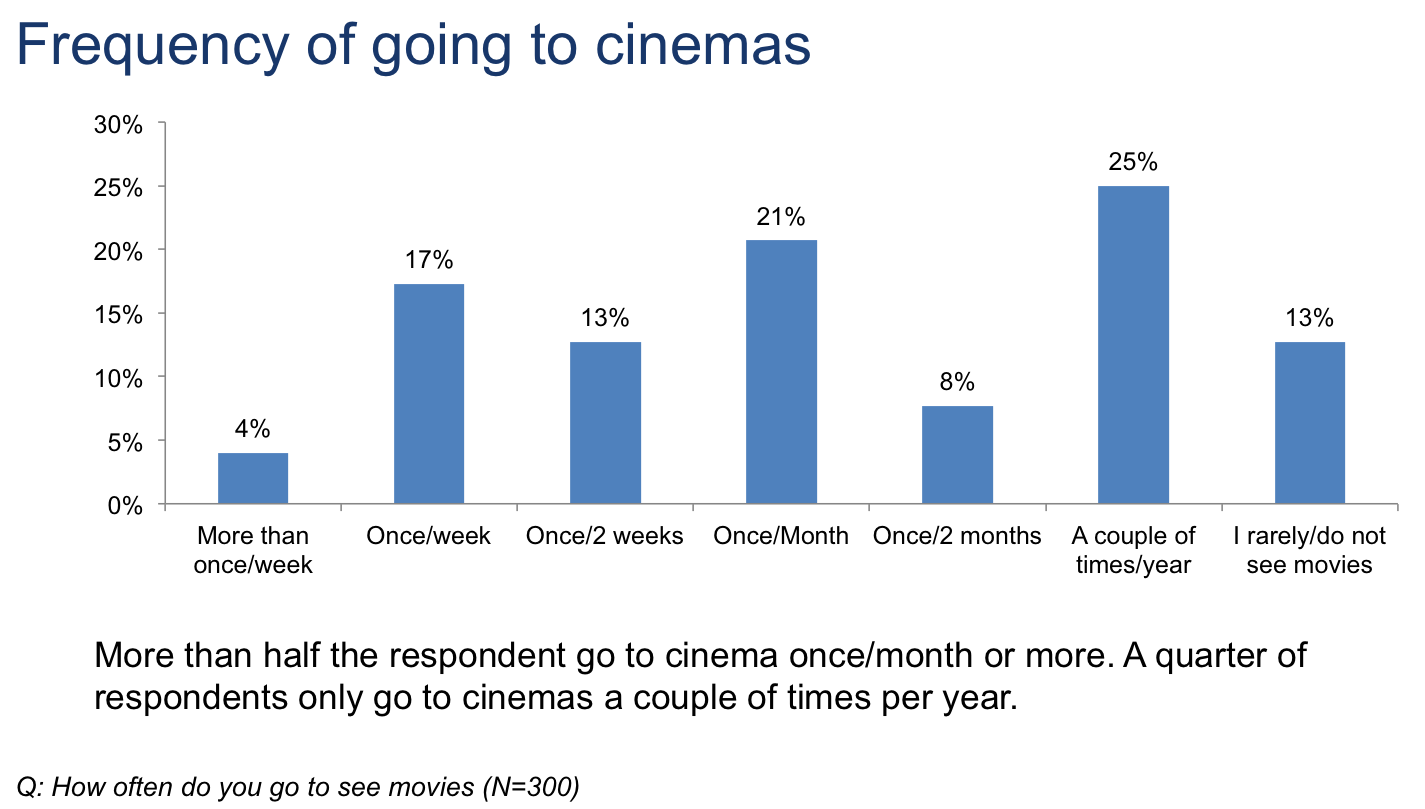
\includegraphics[scale=0.7]{Figs/Static.png}
    \caption{Bảng số liệu thống kê Tần suất ra rạp xem phim của người Việt năm 2022}
\end{figure}
Với sự gia tăng nhu cầu xem phim và ngày càng quan trọng của việc tìm kiếm thông tin chất lượng về các bộ phim, việc xây dựng một trang web review phim chất lượng và tin cậy trở thành một nhiệm vụ quan trọng. Nắm bắt được những nhu cầu thực tế của người dùng không cần bỏ nhiều thời gian nhưng vẫn có thể hiểu được ý nghĩa bộ phim. 

Hiện nay, có rất nhiều nguồn thông tin về phim trực tuyến nhưng việc tìm kiếm và lọc thông tin này để tìm ra những bộ phim phù hợp và đáng xem vẫn là một vấn đề khó khăn. Người dùng thường phải dành nhiều thời gian và công sức để tìm kiếm thông tin về phim, cũng như dựa vào ý kiến của người khác để đưa ra quyết định xem phim.

Để giải quyết vấn đề này, đồ án này đề xuất một ứng dụng web quản lý thông tin về phim, cung cấp các tính năng tìm kiếm, xem thông tin chi tiết và đánh giá phim. Ứng dụng sẽ giúp người dùng dễ dàng tìm kiếm các bộ phim theo tiêu chí như thể loại, năm sản xuất và tên phim. Đồng thời, ứng dụng cũng đề xuất các bộ phim dựa trên sở thích cá nhân của người dùng, giúp họ khám phá thêm nhiều bộ phim mới và đáng chú ý.

Bằng cách áp dụng các công nghệ và công cụ phát triển phần mềm hiện đại, chúng mình hy vọng rằng ứng dụng sẽ giúp người dùng tiết kiệm thời gian và nỗ lực trong việc tìm kiếm và khám phá thế giới điện ảnh, đồng thời mang đến trải nghiệm xem phim tốt hơn.
\subsection{Ý nghĩa của đồ án}
Đồ án này mang lại nhiều ý nghĩa quan trọng từ các khía cạnh khác nhau. Dưới đây là một số ý nghĩa chính mà đồ án đem lại:
\begin{itemize}
    \item \textbf{Tiện lợi cho người dùng}: Ứng dụng web quản lý thông tin về phim sẽ mang lại tiện ích và thuận lợi cho người dùng trong việc tìm kiếm, xem thông tin chi tiết và đánh giá phim. Người dùng có thể dễ dàng tìm kiếm các bộ phim theo tiêu chí mong muốn, tiết kiệm thời gian và nỗ lực trong việc khám phá thế giới điện ảnh.
    \item \textbf{Cung cấp thông tin đa dạng về phim}: Với bộ dữ liệu với hơn \textbf{2000} phim thuộc nhiều thể loại, ứng dụng giúp người dùng tiếp cận với nhiều thể loại phim và nhiều bộ phim đáng chú ý. Điều này sẽ mở rộng khả năng khám phá và tìm kiếm các bộ phim mới, mang đến trải nghiệm xem phim đa dạng và phong phú.
    \item \textbf{Đề xuất phim dựa trên sở thích cá nhân}:  Ứng dụng sẽ sử dụng thông tin về sở thích cá nhân của người dùng để đề xuất các bộ phim phù hợp. Điều này giúp người dùng khám phá thêm nhiều bộ phim mới và đáng chú ý, mở rộng khả năng xem phim và tận hưởng những trải nghiệm mới.
    \item \textbf{Áp dụng các công nghệ phát triển phần mềm}: Đồ án này sử dụng các công nghệ và công cụ phát triển phần mềm hiện đại như Spring Boot, PostgreSQL và các thư viện phổ biến như Thymeleaf và Bootstrap. Việc áp dụng và tiếp cận các công nghệ này giúp nâng cao kỹ năng và hiểu biết về phát triển ứng dụng web.
    \item \textbf{Tiềm năng phát triển và ứng dụng trong thực tế}:Đồ án mang lại tiềm năng phát triển và ứng dụng rộng rãi trong thực tế. Các tính năng và công nghệ đã sử dụng có thể được mở rộng và tùy chỉnh để phục vụ cho các ứng dụng quản lý thông tin khác, không chỉ riêng trong lĩnh vực điện ảnh.
\end{itemize}
Qua việc thực hiện đồ án này, chúng mình hy vọng rằng sẽ đem lại giá trị thực tiễn và đáp ứng được nhu cầu của người dùng trong việc tìm kiếm và khám phá thế giới điện ảnh một cách tiện lợi và hấp dẫn.


\subsection{ Khảo sát các công trình liên quan}
\subsubsection{Các công trình}
Trước khi triển khai đồ án, chúng mình đã tiến hành khảo sát và nghiên cứu các công trình liên quan trong lĩnh vực quản lý thông tin phim. Dưới đây là một số công trình quan trọng mà chúng mình đã khảo sát:
\begin{itemize}
    \item \textbf{IMDb (Internet Movie Database)}: là một trong những công trình nổi tiếng và phổ biến nhất trong việc quản lý thông tin về phim trực tuyến. 
    \item \textbf{Rotten Tomatoes}: là một trang web đánh giá phim và chương trình truyền hình.
    \item \textbf{Letterboxd}: Letterboxd là một mạng xã hội cho phép người dùng tạo và chia sẻ danh sách phim yêu thích, đánh giá và nhận xét phim, và tương tác với cộng đồng người dùng khác.
    \item \textbf{Netflix, Amazon Prime, và các dịch vụ phát trực tuyến khác}: Các dịch vụ phát trực tuyến như Netflix và Amazon Prime cung cấp nền tảng quản lý thông tin phim cho người dùng. 
\end{itemize}
Thông qua việc khảo sát các công trình liên quan, chúng mình đã thu thập được nhiều thông tin và ý kiến quý giá về các tính năng, giao diện, và quản lý thông tin phim. Điều này đã giúp chúng mình xác định được những yếu tố quan trọng và đặc điểm độc đáo mà chúng mình muốn tích hợp vào đồ án của mình, từ đó nâng cao trải nghiệm người dùng và giá trị của ứng dụng.
\subsubsection{Những thiếu sót của những công trình hiện có}
Trong quá trình khảo sát và nghiên cứu các công trình liên quan, chúng mình đã nhận thấy một số điểm yếu của các website quản lý thông tin phim hiện có. Dưới đây là những điểm yếu quan trọng mà chúng mình đã rút ra từ các công trình khảo sát:
\begin{itemize}
    \item \textbf{Không có trailer phim}: Một số website không cung cấp trailer phim đi kèm với thông tin chi tiết của bộ phim. Điều này làm giảm khả năng người dùng có cái nhìn trực quan và cảm nhận về nội dung, phong cách và hiệu quả truyền đạt của phim. Thiếu trailer có thể khiến người dùng cảm thấy khó lòng đánh giá chính xác về sự hấp dẫn của một bộ phim.
    \begin{figure}[H]
        \centering
        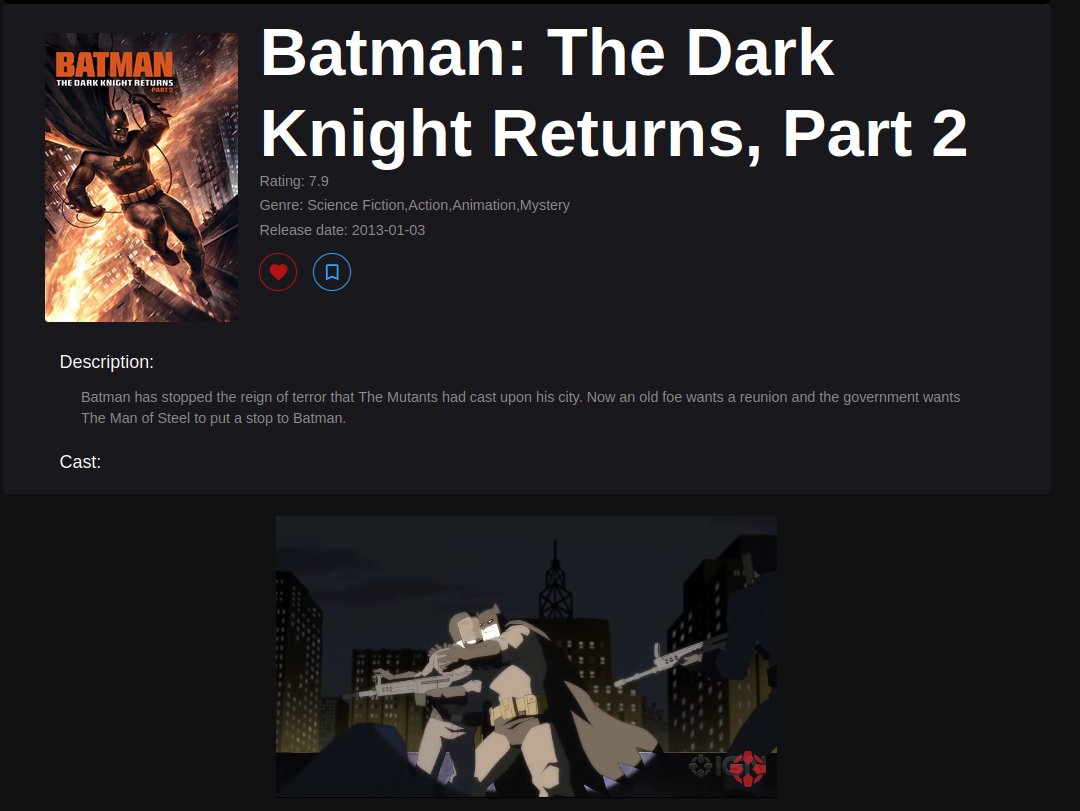
\includegraphics[scale=0.4]{Figs/Trailer_Review.png}
        \caption{Spring Movie Review hỗ trợ Trailer}
    \end{figure}
    \item \textbf{Hệ thống đánh giá không tin cậy}: Một số website có hệ thống đánh giá phim không đáng tin cậy hoặc dễ bị ảnh hưởng bởi các đánh giá không chính xác hoặc thiên vị. Điều này có thể gây ra sự bất mãn và đánh lạc hướng người dùng trong việc chọn lựa phim.
    \item \textbf{Thiếu hệ thống recommend (gợi ý)}: Một số website không có hệ thống recommend (gợi ý) phim dựa trên sở thích và lịch sử xem phim của người dùng. Điều này làm mất đi cơ hội để người dùng khám phá các bộ phim mới và đa dạng hơn, dựa trên các tiêu chí cá nhân và sở thích của họ.
\end{itemize}
Đồ án của chúng mình sẽ tập trung vào giải quyết những điểm yếu này bằng cách cung cấp trailer phim, thông tin về diễn viên (Cast) và xây dựng hệ thống recommend (gợi ý) phim thông minh, từ đó nâng cao trải nghiệm và sự hài lòng của người dùng.
\section{Lý thuyết, các công cụ sử dụng để giải quyết vấn đề}
\subsection{Lý thuyết cơ sở}

Trong phần này, chúng ta sẽ xem xét những lý thuyết cơ sở và khái niệm quan trọng liên quan đến đồ án. Những lý thuyết này cung cấp nền tảng lý thuyết và hiểu biết cần thiết để xây dựng và triển khai ứng dụng quản lý thông tin phim. Dưới đây là một số lý thuyết cơ sở quan trọng:
\begin{itemize}
    \item \textbf{Cơ sở dữ liệu quan hệ (Relational Database)}: Đồ án sử dụng cơ sở dữ liệu PostgreSQL, một hệ quản trị cơ sở dữ liệu quan hệ phổ biến. Chúng ta sẽ xem xét các khái niệm cơ bản của cơ sở dữ liệu quan hệ, bao gồm các bảng, quan hệ, khóa chính và khóa ngoại. Chúng ta cũng sẽ tìm hiểu cách sử dụng SQL để truy vấn và thao tác dữ liệu trong cơ sở dữ liệu.

    \item \textbf{Mô hình hóa dữ liệu (Data Modeling)}: Để thiết kế cơ sở dữ liệu phim, chúng mình sẽ áp dụng các nguyên tắc và kỹ thuật mô hình hóa dữ liệu. Chúng ta sẽ xem xét các mô hình dữ liệu như mô hình thực thể-liên kết và mô hình quan hệ. Chúng ta cũng sẽ tìm hiểu cách xác định các thực thể, mối quan hệ và thuộc tính trong cơ sở dữ liệu phim.

    \item \textbf{Spring Framework và Spring Boot}: Đồ án sử dụng Spring Boot, một framework phát triển ứng dụng Java nhanh chóng và dễ dùng.Tìm hiểu về các thành phần quan trọng của Spring Boot như Dependency Injection, Spring MVC, và Spring Data JPA. Tìm hiểu cách hoạt động của Spring Boot giúp chúng ta xây dựng ứng dụng web dễ dàng và hiệu quả.
    \begin{figure}[H]
        \centering
        
\includegraphics[scale=0.6]{Figs/spring-logo.png}
    \end{figure}
    \item \textbf{Mô hình phát triển MVC (Model-View-Controller)}: Ap dụng mô hình phát triển MVC để tách biệt logic xử lý, hiển thị và quản lý dữ liệu trong ứng dụng của chúng ta. Xây dựng các thành phần Model, View và Controller trong ứng dụng quản lý thông tin phim để đảm bảo tính rõ ràng, dễ bảo trì và mở rộng của mã nguồn.

\end{itemize}

Overall, the Football League Management App will provide a comprehensive solution for managing football leagues, with features designed to streamline administrative tasks, improve communication, and promote fair play and transparency.
\subsection{Các công cụ sử dụng}
Trong phần này, chúng ta sẽ tìm hiểu về các công cụ mà chúng ta sử dụng để giải quyết vấn đề trong đồ án. Các công cụ này cung cấp giải pháp và hỗ trợ cho quá trình phát triển và triển khai ứng dụng quản lý thông tin phim của chúng ta. Dưới đây là một số công cụ quan trọng mà chúng ta sử dụng:
\begin{itemize}
    \item \textbf{IntelliJ IDEA}: là môi trường phát triển tích hợp (IDE) mạnh mẽ và phổ biến dành cho phát triển ứng dụng Java. Chúng ta sử dụng IntelliJ IDEA để viết mã nguồn, quản lý dự án và thực hiện các tác vụ phát triển khác. IDE này cung cấp nhiều tính năng hữu ích như gỡ lỗi, tự động hoàn thành mã, và tích hợp với các công cụ khác.
    \begin{figure}[H]
        \centering
        
\includegraphics[scale=0.15]{Figs/IntelliJ_IDEA_Icon.svg.png}
    \end{figure}

    \item \textbf{PostgreSQL}: PostgreSQL là hệ quản trị cơ sở dữ liệu quan hệ mạnh mẽ, mã nguồn mở. Chúng mình sử dụng PostgreSQL để lưu trữ dữ liệu về phim và các thông tin liên quan. PostgreSQL cung cấp các tính năng bảo mật, khả năng mở rộng và khả năng xử lý dữ liệu phức tạp.
    \item \textbf{Thymeleaf}: Thymeleaf là một engine template đáng tin cậy và mạnh mẽ cho ứng dụng web Java. Chúng ta sử dụng Thymeleaf để tạo và hiển thị các trang HTML động trong ứng dụng. Thymeleaf kết hợp tốt với Spring Framework và cung cấp các tính năng như thực hiện biểu thức notation, lặp lại dữ liệu và binding dữ liệu.
    \item \textbf{Bootstrap}: Bootstrap là một framework CSS phổ biến và mạnh mẽ để thiết kế giao diện web responsive. Chúng mình sử dụng Bootstrap để xây dựng giao diện người dùng thân thiện và tương thích với nhiều thiết bị và kích thước màn hình khác nhau. Bootstrap cung cấp các components, lớp và kiểu patterns để tạo giao diện hấp dẫn và chuyên nghiệp.
\end{itemize}
\section{Phân tích, thiết kế, hiện thực hệ thống}
\subsection{Phân tích yêu cầu}
Trước khi tiến hành thiết kế và hiện thực hệ thống quản lý thông tin phim, chúng phân tích cẩn thận các yêu cầu chức năng và phi chức năng của đồ án. Quá trình phân tích này giúp chúng ta hiểu rõ hơn về các tính năng cần có và các yêu cầu mà hệ thống phải đáp ứng. Dưới đây là một số phân tích chính:
\subsubsection{Functional Requirements}
\begin{itemize}
    \item \textbf{Đăng nhập và đăng ký người dùng}: Cho phép người dùng tạo tài khoản và đăng nhập vào hệ thống.
    \item \textbf{Thêm, xóa, sửa phim}: Cho phép Admin có quyền thêm, xóa, sửa dữ liệu phim.
    \item \textbf{Tìm kiếm phim}: Cung cấp khả năng tìm kiếm và lọc phim dựa trên các tiêu chí như tên phim, thể loại, diễn viên, đạo diễn, năm sản xuất, v.v.
    \item \textbf{Xem chi tiết phim}: Hiển thị thông tin chi tiết về một phim cụ thể bao gồm mô tả, diễn viên, đạo diễn, thể loại, đánh giá, v.v.
    \item \textbf{Hỗ trợ Trailer phim}: Hiển thị trailer cho phim giúp người dùng có cái nhìn tổng quát về phim.
    \item \textbf{Thêm phim vào danh sách yêu thích}: Cho phép người dùng thêm phim vào danh sách yêu thích của họ để theo dõi và truy cập nhanh vào những phim mà họ quan tâm.
    \item \textbf{Tính năng Recommend phim}: Sử dụng các thuật toán để đánh giá và đề xuất những phim mà người dùng thích, Hiển thị những phim phù hợp với từng đối tượng người dùng.
    \item \textbf{Đánh giá phim}: Cho phép người dùng xem và đọc những đánh giá do người dùng khác thực hiện, cung cấp hệ thống chấm điểm cho từng phim.
\end{itemize}
\subsubsection{Non-Functional Requirements}
Ngoài các chức năng chính, chúng ta cũng cần xem xét các yêu cầu phi chức năng mà hệ thống cần đáp ứng. Điều này có thể bao gồm:
\begin{itemize}
    \item \textbf{Bảo mật}: Đảm bảo rằng chỉ người dùng đã đăng nhập mới có thể truy cập vào các chức năng và thông tin nhạy cảm.
    \item \textbf{Tính khả dụng}: Hệ thống phải có thời gian phản hồi nhanh chóng và khả năng xử lý đồng thời nhiều yêu cầu từ người dùng.
    \item \textbf{Giao diện người dùng thân thiện}: Thiết kế giao diện người dùng đơn giản, dễ sử dụng và thân thiện để người dùng có trải nghiệm tốt khi sử dụng hệ thống.
\end{itemize}
\subsubsection{Use Case Diagram}
Use case là một công cụ quan trọng trong phân tích yêu cầu. Chúng ta xác định các use case chính và các tác nhân liên quan, đồng thời xác định các tương tác giữa tác nhân và hệ thống. Use case giúp chúng ta hiểu rõ hơn về cách người dùng sẽ sử dụng hệ thống và cung cấp cơ sở cho việc thiết kế hệ thống.
\begin{figure}[H]
    \centering
    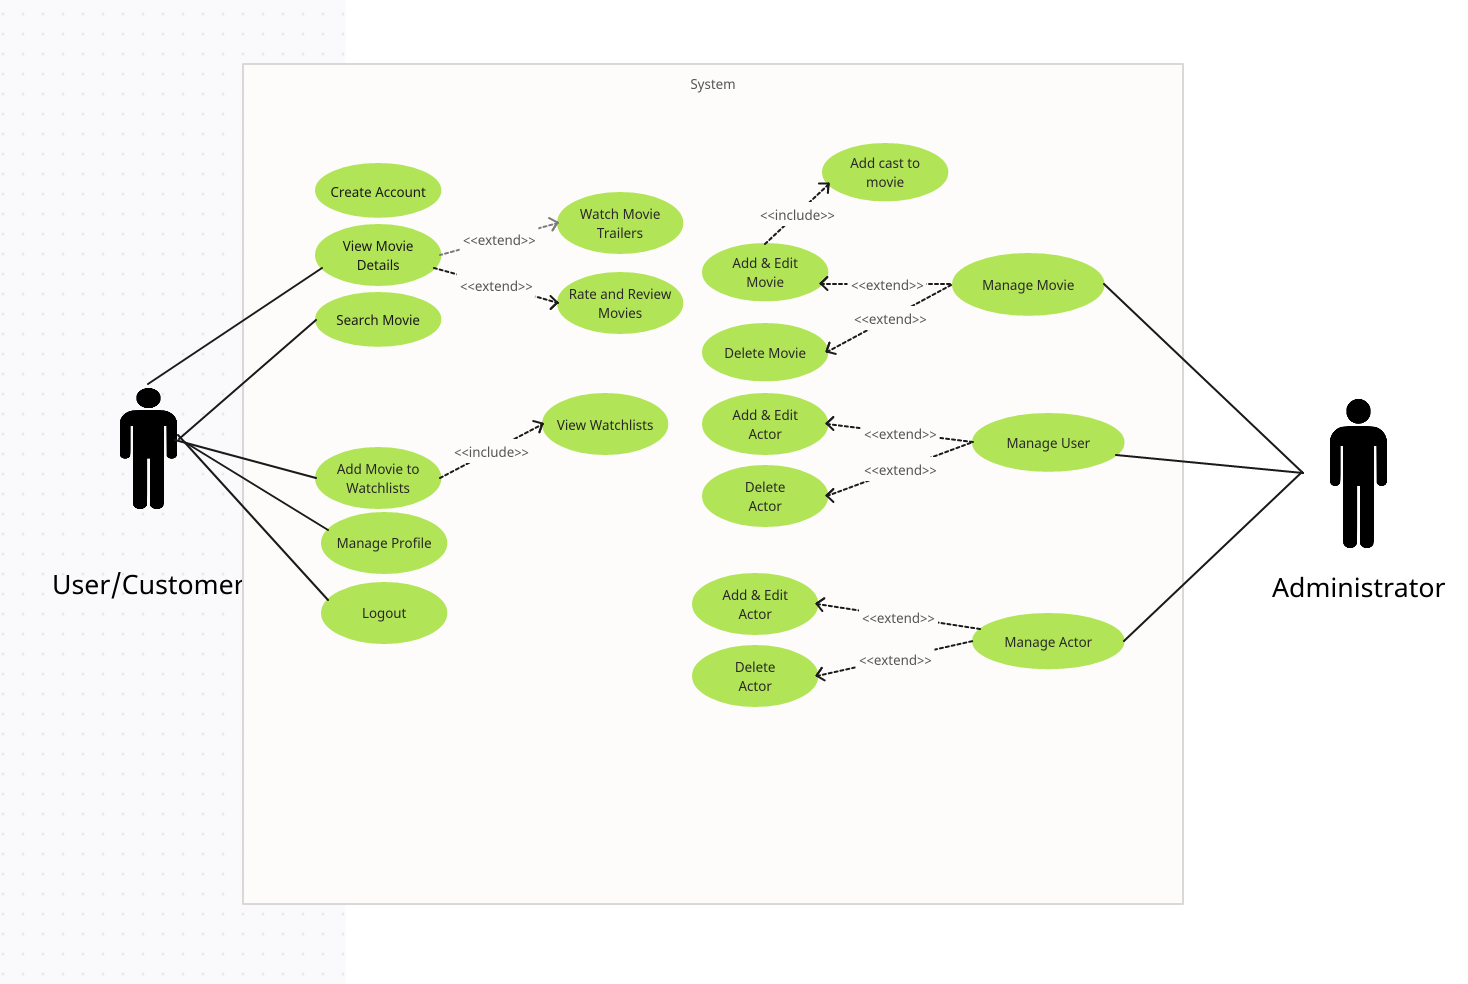
\includegraphics[scale=0.45]{Figs/Use_case.png}
    \caption{Spring Movie Review - Use Case Diagram}
\end{figure}
\subsection{Thiết kế hệ thống}
\subsubsection{Kiến trúc hệ thống}
\begin{itemize}
    \item Kiến trúc ba lớp (Three-Tier Architecture):  Hệ thống quản lý phim có thể được thiết kế theo kiến trúc ba lớp, bao gồm:
    \begin{enumerate}
        \item Presentation Layer (Lớp Trình bày): Đây là giao diện người dùng, nơi người dùng tương tác với hệ thống. Các yêu cầu từ người dùng được gửi đến lớp Application để xử lý.
        \begin{figure}[H]
            \centering
            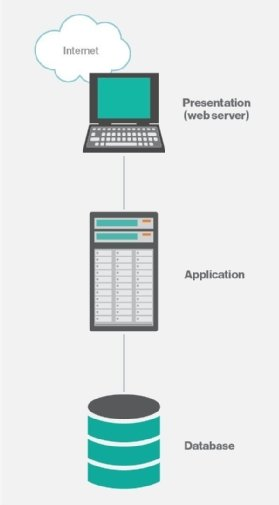
\includegraphics[scale=0.5]{Figs/three_tier_arch_half_column_mobile.jpg}
            \caption{Three-Tier Architecture}
        \end{figure}
        \item Application Layer:
            \begin{itemize}
                \item     Controllers: Đây là thành phần chịu trách nhiệm nhận các yêu cầu từ phía người dùng thông qua các API và điều hướng chúng đến các phương thức tương ứng để xử lý. Controllers cũng có nhiệm vụ truyền dữ liệu giữa người dùng và lớp Application.

                \item  Services: Đây là thành phần chứa các luật logic nghiệp vụ của hệ thống. Lớp Application sẽ sử dụng các service để thực hiện các chức năng như thêm, sửa, xóa phim, quản lý người dùng, và thực hiện các tác vụ khác liên quan đến quản lý phim.
                
                \item  Repositories: Đây là thành phần sử dụng để truy cập và thao tác dữ liệu trong cơ sở dữ liệu. Lớp Application sẽ giao tiếp với các repositories để lấy dữ liệu từ cơ sở dữ liệu, thực hiện các truy vấn và cập nhật dữ liệu khi cần thiết.
            
                \item  Models: Đây là các đối tượng mô hình hóa dữ liệu trong hệ thống. Lớp Application sẽ sử dụng các models để truyền và xử lý dữ liệu trong quá trình xử lý.
            \end{itemize}

            Lớp Application sẽ làm cầu nối giữa các thành phần khác nhau trong hệ thống và đảm bảo rằng các yêu cầu được xử lý đúng theo luật logic nghiệp vụ của ứng dụng. Nó cũng sẽ quản lý việc truy cập và cập nhật dữ liệu thông qua việc sử dụng các repositories.

            \item Data Layer (Lớp Dữ liệu): Đây là cơ sở dữ liệu nơi lưu trữ thông tin về các phim, người dùng, diễn viên và các thông tin liên quan khác.

        \end{enumerate}
    \item Cơ sở dữ liệu PostgreSQL: Hệ thống quản lý phim sử dụng cơ sở dữ liệu PostgreSQL để lưu trữ và quản lý dữ liệu. PostgreSQL được chọn vì tính bảo mật, độ tin cậy và khả năng mở rộng.
    \item RESTful API: Hệ thống cung cấp một RESTful API để cho phép các ứng dụng khác (ví dụ: ứng dụng di động) tương tác với dữ liệu của hệ thống quản lý phim. API này cung cấp các endpoint để thực hiện các hoạt động như lấy danh sách phim, thêm phim mới, chỉnh sửa thông tin phim, và xóa phim.
    \item Hệ thống xếp hạng và đề xuất (Recommendation System): Để cung cấp trải nghiệm cá nhân hóa cho người dùng, hệ thống quản lý phim có thể tích hợp một hệ thống xếp hạng và đề xuất. Hệ thống này sẽ phân tích dữ liệu về lịch sử xem phim và sở thích của người dùng để đề xuất những phim tương tự hoặc phù hợp với sở thích của họ.
    \item Bảo mật và quản lý người dùng: Hệ thống có các biện pháp bảo mật để đảm bảo an toàn thông tin và quyền riêng tư của người dùng. Điều này có thể bao gồm xác thực người dùng, quản lý phiên đăng nhập, mã hóa dữ liệu và kiểm soát quyền truy cập.
    \item Hiệu năng và mở rộng: Hệ thống được thiết kế để đảm bảo hiệu năng ổn định và khả năng mở rộng. Các biện pháp như caching, tối ưu hóa cơ sở dữ liệu và triển khai phân tán có thể được sử dụng để đáp ứng tải lượng sử dụng cao và mở rộng hệ thống theo nhu cầu.
\end{itemize}
\subsubsection{Mô hình dữ liệu}
Trong phần "Mô hình dữ liệu", chúng ta sẽ mô tả cấu trúc dữ liệu và mối quan hệ giữa các thành phần trong hệ thống quản lý phim. Dưới đây là mô hình dữ liệu cơ bản cho hệ thống:
\begin{figure}[H]
    \centering
    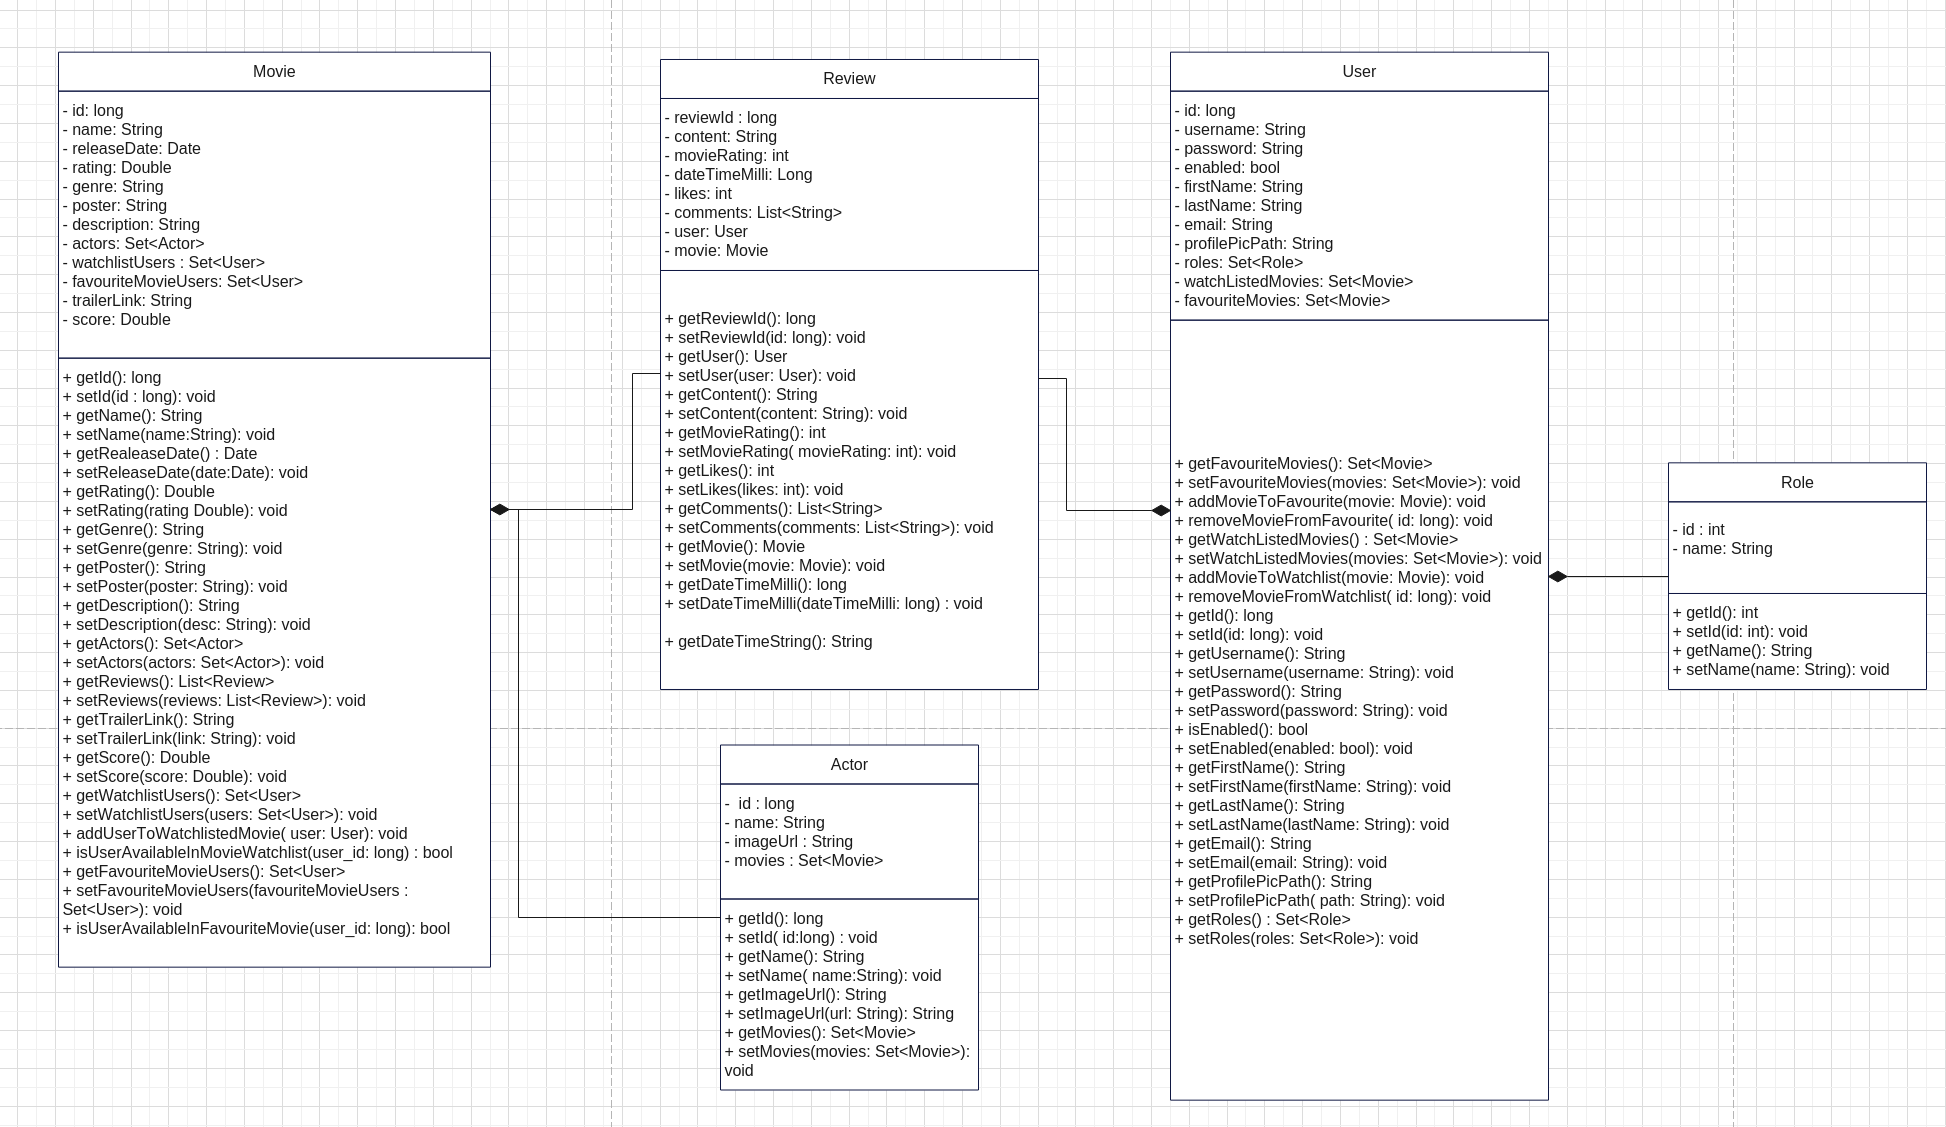
\includegraphics[scale=0.35]{Figs/classDiagram.png}
    \caption{Class Diagram}
\end{figure}
\subsubsection{Giao diện người dùng}
Khi thiết kế giao diện cho hệ thống quản lý phim, chúng ta có thể định nghĩa một số ràng buộc để đảm bảo tính hợp lý và tương thích của giao diện. Dưới đây là một số ràng buộc cơ bản:
\begin{itemize}
    \item     Responsive Design: Giao diện cần được thiết kế linh hoạt và tương thích trên các thiết bị khác nhau, bao gồm máy tính, điện thoại di động và máy tính bảng. Giao diện phải có khả năng thích ứng với các kích thước màn hình khác nhau và tự động điều chỉnh để hiển thị một cách tối ưu trên từng thiết bị.

    \item Sử dụng giao diện thân thiện người dùng: Giao diện cần được thiết kế để đảm bảo tính thân thiện và dễ sử dụng cho người dùng. Các thành phần giao diện như nút, trường nhập liệu, menu, và liên kết phải được đặt một cách rõ ràng, dễ nhìn và dễ tương tác.

    \item Đảm bảo tính nhất quán: Giao diện của các trang và màn hình trong hệ thống cần có một hình thức nhất quán, bao gồm việc sử dụng cùng một kiểu chữ, màu sắc, hình ảnh, biểu tượng và các yếu tố thiết kế khác. Điều này giúp người dùng dễ dàng điều hướng và có trải nghiệm liền mạch trên toàn bộ hệ thống.

    \item Kiểm soát dữ liệu đầu vào: Giao diện cần kiểm tra và kiểm soát dữ liệu đầu vào từ người dùng để đảm bảo tính hợp lệ và bảo mật. Kiểm tra đầu vào và xử lý lỗi giúp ngăn chặn các lỗi nhập liệu không mong muốn và bảo vệ hệ thống khỏi các cuộc tấn công.
    \begin{figure}[H]
        \centering
        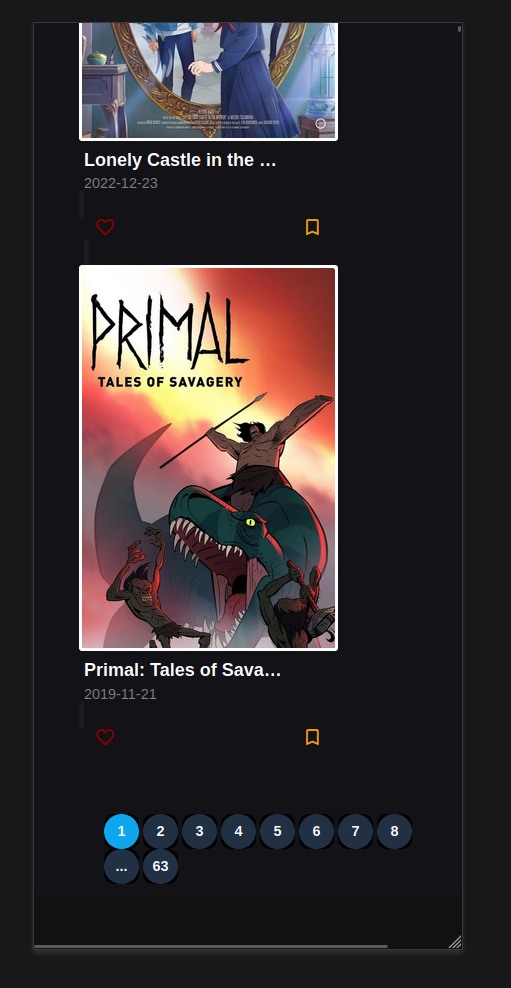
\includegraphics[scale=0.45]{Figs/phone_screen.png}
        \caption{Giao diện Spring Movie Review trên điện thoại}
    \end{figure}
    \item Hiển thị thông tin hợp lý: Giao diện cần hiển thị thông tin một cách hợp lý và có tổ chức. Thông tin cần được sắp xếp một cách logic và dễ đọc, đồng thời tránh hiển thị quá nhiều thông tin một lúc để tránh làm rối mắt người dùng.

    \item Sử dụng các phương pháp tương tác thích hợp: Giao diện cần sử dụng các phương pháp tương tác thích hợp như nút bấm, trường nhập liệu, menu thả xuống, và các thao tác kéo và thả để tạo ra trải nghiệm người dùng tốt nhất.
\end{itemize}
\subsubsection{Quy trình xử lý}
Đưa ra mô tả chi tiết về quy trình xử lý cho mỗi use case, từ khi người dùng thực hiện hành động cho đến khi hệ thống thực hiện các tác vụ tương ứng. Dưới đây là các biểu đồ hoạt động (activity diagram) cho một số use case.
\begin{figure}[H]
    \centering
    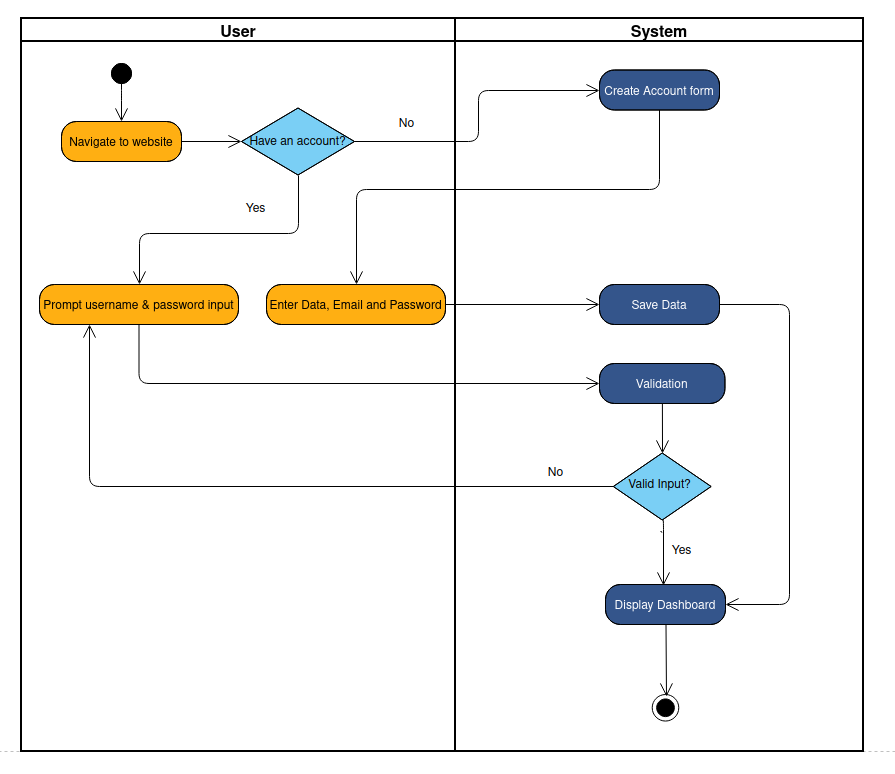
\includegraphics[scale=0.7]{Figs/login_activity.png}
    \caption{Spring Movie Review Login and Registration Activity}
\end{figure}
\begin{figure}[H]
    \centering
    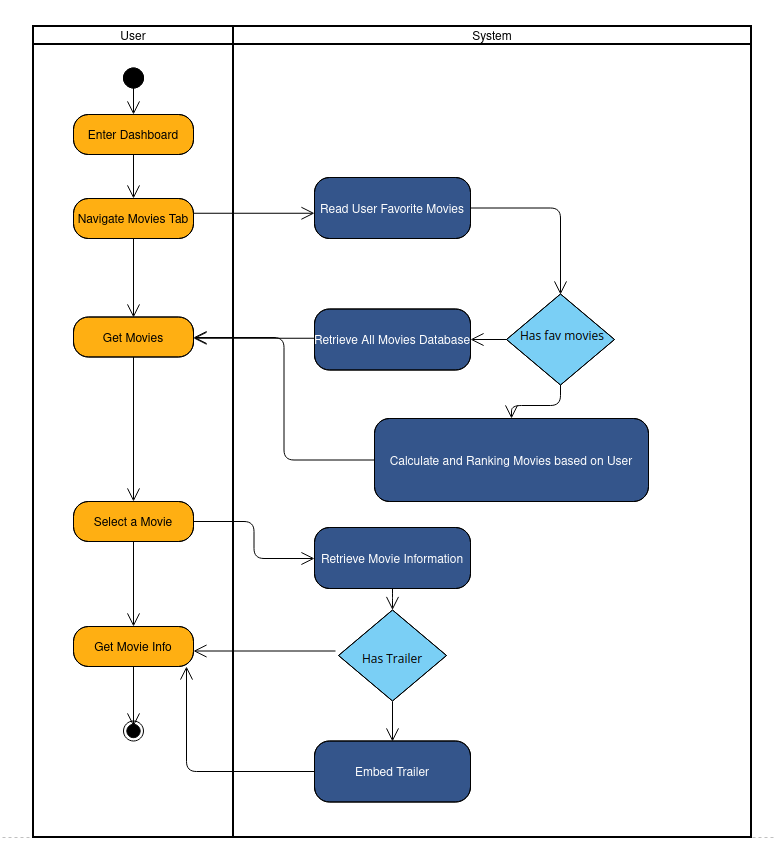
\includegraphics[scale=0.7]{Figs/Get_Movie_Activity.png}
    \caption{Spring Movie Review Get Movie Information Activity}
\end{figure}
\begin{figure}[H]
    \centering
    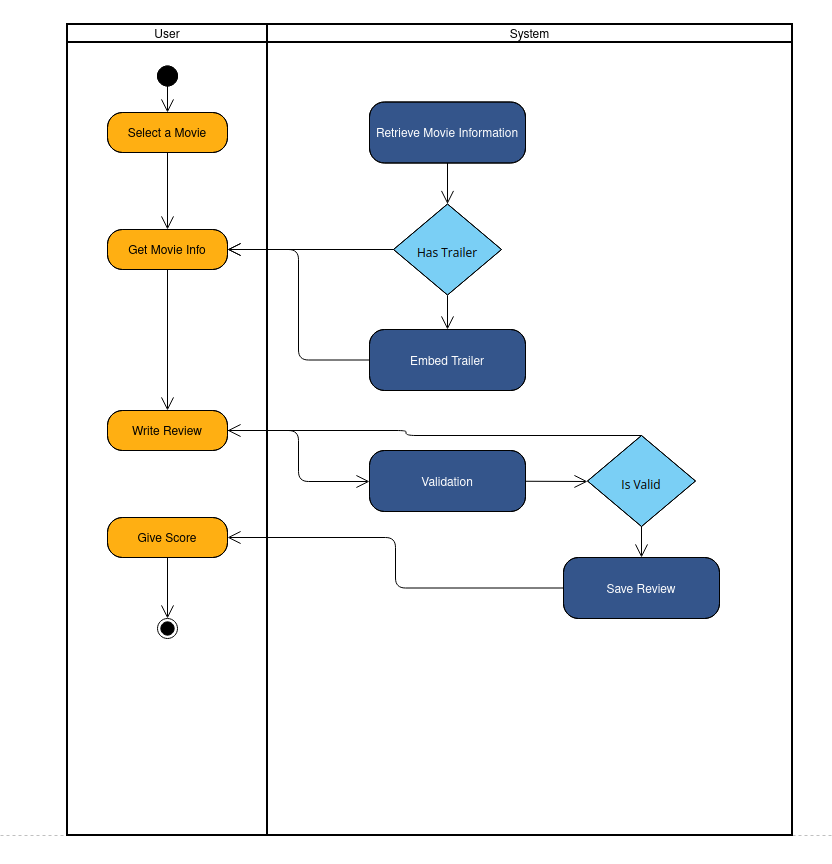
\includegraphics[scale=0.7]{Figs/Review_Activity.png}
    \caption{Spring Movie Review Write Review Activity}
\end{figure}
\subsubsection{Cơ sở dữ liệu}
Đưa ra thiết kế cụ thể về cơ sở dữ liệu trong hệ thống, bao gồm các bảng, trường, ràng buộc, và quan hệ giữa chúng. Sử dụng các biểu đồ mô hình dữ liệu như biểu đồ Entity-Relationship (ER diagram) để trình bày cấu trúc dữ liệu của hệ thống.
\begin{figure}[H]
    \centering
    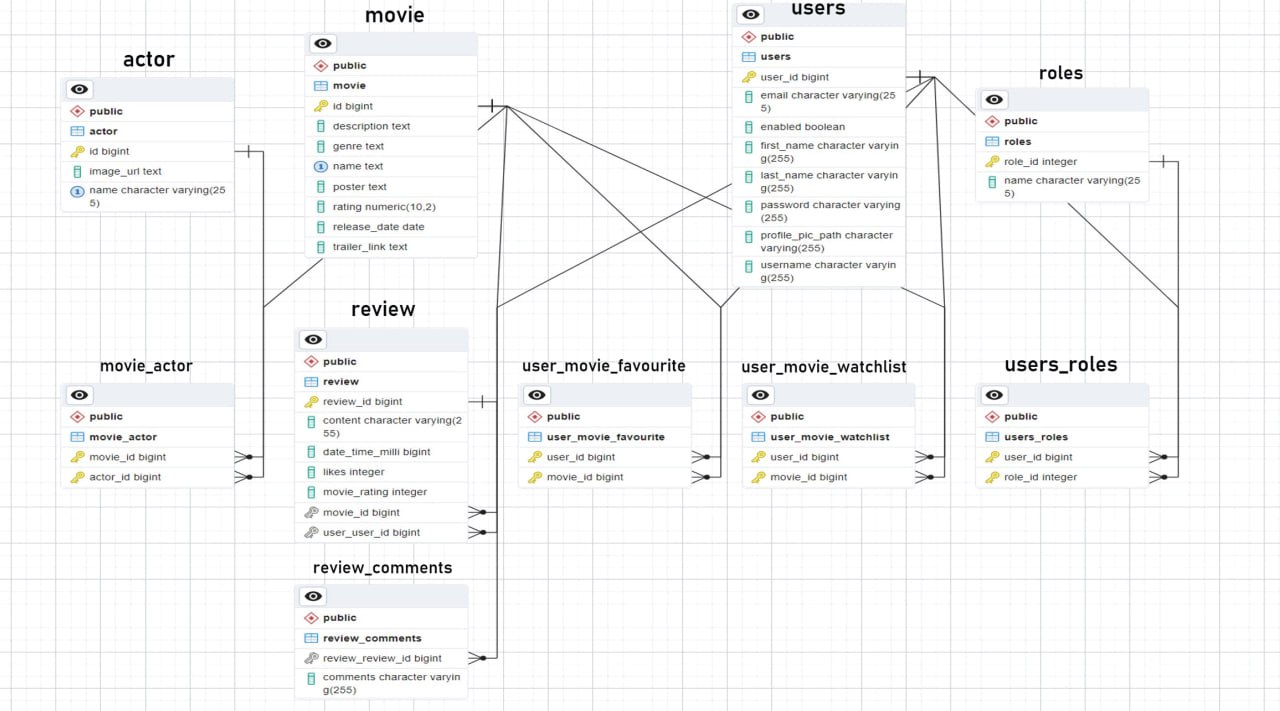
\includegraphics[scale=1.5]{Figs/database.jpg}
    \caption{Spring Movie Review - ERD}
\end{figure}
\subsubsection{Security Constraints}
Bảo mật là một yếu tố quan trọng trong việc xây dựng hệ thống quản lý phim để đảm bảo an toàn thông tin và bảo vệ quyền riêng tư của người dùng. Dưới đây là một số biện pháp bảo mật quan trọng được áp dụng trong hệ thống:
\begin{itemize}
    \item Quản lý quyền truy cập: Hệ thống cần áp dụng các cơ chế quản lý quyền truy cập nhằm đảm bảo chỉ những người dùng có quyền được phép mới có thể truy cập vào các chức năng và dữ liệu quan trọng. Điều này có thể được đạt được thông qua việc thiết lập vai trò và quyền hạn cho từng người dùng trong hệ thống.

    \item Mã hóa dữ liệu: Để đảm bảo an toàn thông tin, dữ liệu quan trọng như thông tin người dùng, đăng nhập và mật khẩu cần được mã hóa trước khi lưu trữ trong cơ sở dữ liệu. Điều này giúp ngăn chặn việc đánh cắp thông tin nhạy cảm trong trường hợp có xâm nhập vào hệ thống.
    \item Bảo vệ quyền riêng tư: Hệ thống cần tuân thủ các quy định về bảo vệ quyền riêng tư của người dùng. Điều này bao gồm việc xác định và bảo vệ các thông tin riêng tư của người dùng, không tiết lộ thông tin cá nhân không cần thiết và tuân thủ các quy định pháp luật liên quan đến bảo vệ quyền riêng tư.
\end{itemize}
\subsubsection{Ràng buộc Hiệu năng}
Hiệu năng và mở rộng là những yếu tố quan trọng trong việc xây dựng hệ thống quản lý phim để đảm bảo rằng hệ thống hoạt động một cách hiệu quả và có khả năng mở rộng khi tải lượng sử dụng tăng cao. Dưới đây là một số biện pháp để đảm bảo hiệu năng ổn định và khả năng mở rộng của hệ thống:
\begin{itemize}
    \item Sử dụng bộ nhớ cache: Bộ nhớ cache giúp lưu trữ các dữ liệu phổ biến và kết quả truy vấn để tăng tốc độ truy cập dữ liệu. Bằng cách sử dụng bộ nhớ cache, ta có thể giảm thiểu số lần truy vấn cơ sở dữ liệu và cải thiện hiệu năng của hệ thống.

    \item Tối ưu hóa truy vấn cơ sở dữ liệu: Đảm bảo rằng các truy vấn cơ sở dữ liệu được viết một cách hiệu quả và tối ưu. Sử dụng các chỉ mục, tối ưu hóa câu truy vấn và sử dụng các phương pháp tối ưu hóa khác để giảm thiểu thời gian truy vấn và tăng tốc độ xử lý dữ liệu.

    \item Triển khai cơ chế mở rộng: Khi tải lượng sử dụng tăng cao, hệ thống cần có khả năng mở rộng để xử lý được số lượng người dùng và yêu cầu tăng. Sử dụng cơ chế phân tán và cân bằng tải để chia nhỏ công việc và phân phối tải trọng trên nhiều máy chủ hoặc các thành phần của hệ thống.

    \item Đo lường và tối ưu hiệu năng: Định kỳ đo lường và kiểm tra hiệu năng của hệ thống để phát hiện các vấn đề và điều chỉnh các thành phần cần thiết. Tối ưu hóa các thành phần yếu để đạt được hiệu suất tốt nhất và đảm bảo rằng hệ thống có thể đáp ứng được yêu cầu của người dùng.
\end{itemize}
\subsection{Hiện thực hệ thống}
\begin{itemize}
    \item Triển khai cơ sở dữ liệu: Sử dụng cơ sở dữ liệu PostgreSQL đã được đề cập trước đó, thiết lập và triển khai cơ sở dữ liệu để lưu trữ thông tin về phim, người dùng, đánh giá và các dữ liệu khác liên quan.

    \item Xây dựng backend: Sử dụng Spring Boot framework, triển khai các lớp controller, service và repository để xử lý các yêu cầu từ phía người dùng và tương tác với cơ sở dữ liệu. Các chức năng như thêm, sửa, xóa phim, đánh giá, tìm kiếm và khớp phim sẽ được triển khai trong các lớp tương ứng.

    \item Xây dựng giao diện người dùng: Sử dụng HTML, CSS và JavaScript, xây dựng giao diện người dùng cho hệ thống quản lý phim. Đảm bảo rằng giao diện có thiết kế thân thiện, dễ sử dụng và tuân thủ các nguyên tắc thiết kế đã được đề ra trong phần trước.

    \item Tích hợp các API và dịch vụ bên ngoài: Nếu cần thiết, ta có thể tích hợp các API và dịch vụ bên ngoài để mở rộng chức năng của hệ thống. Ví dụ, ta có thể tích hợp API của các nhà cung cấp phim để lấy thông tin chi tiết về phim hoặc tích hợp dịch vụ thanh toán để xử lý thanh toán mua vé.
    \begin{figure}[H]
        \centering
        
\includegraphics[scale=0.7]{Figs/TMDB.jpg}
        \caption{The Movie Database API}
    \end{figure}
    \item Kiểm thử và debug: Trong quá trình triển khai và triển khai, tiến hành kiểm thử hệ thống để đảm bảo tính ổn định và đúng đắn của các chức năng. Sử dụng các phương pháp kiểm thử như kiểm thử đơn vị, kiểm thử tích hợp và kiểm thử hệ thống để đảm bảo chất lượng của hệ thống.

    \item Theo dõi và bảo trì: Sau khi hệ thống được triển khai, theo dõi và duy trì hoạt động của nó. Đảm bảo rằng hệ thống hoạt động ổn định, xử lý các yêu cầu của người dùng một cách hiệu quả và không gặp lỗi. Nếu có lỗi hoặc vấn đề xảy ra, tiến hành khắc phục và bảo trì hệ thống để đảm bảo sự liên tục và tin cậy.
\end{itemize}
\section{Thử nghiệm, đánh giá kết quả, phân tích}
\subsection{Thử nghiệm}
Tiến hành thử nghiệm hệ thống theo hai phương pháp chính là Black Box Testing và White Box Testing.
\subsubsection{Kiểm thử hộp đen (Black Box Testing)}
Trong giai đoạn kiểm thử hộp đen của ứng dụng Spring Movie Review, chúng mình tập trung vào kiểm tra hệ thống từ một góc nhìn bên ngoài mà không quan tâm đến cấu trúc và logic bên trong của nó. Mục tiêu của chúng mình là đảm bảo rằng hệ thống thực hiện đúng các chức năng và yêu cầu được đề ra. Dưới đây là một số hoạt động và kỹ thuật chính mà chúng mình đã áp dụng:
\begin{itemize}
    \item Kiểm tra giá trị biên: chúng mình đã kiểm tra các giá trị biên đầu vào để đảm bảo rằng hệ thống xử lý chúng một cách chính xác. Ví dụ, chúng mình đã thử nghiệm với các giá trị đầu vào tối thiểu và tối đa cho các trường thông tin phim và người dùng, và kiểm tra xem hệ thống xử lý đúng các giá trị này hay không.
    
    \item Kiểm tra hiệu năng: chúng mình đã kiểm tra hiệu năng của ứng dụng bằng cách thử nghiệm với tải lượng sử dụng tăng dần. chúng mình đã đảm bảo rằng ứng dụng vẫn duy trì hiệu suất ổn định và thời gian phản hồi nhanh chóng trong các tình huống tải lượng cao.
    \begin{figure}[H]
        \centering
        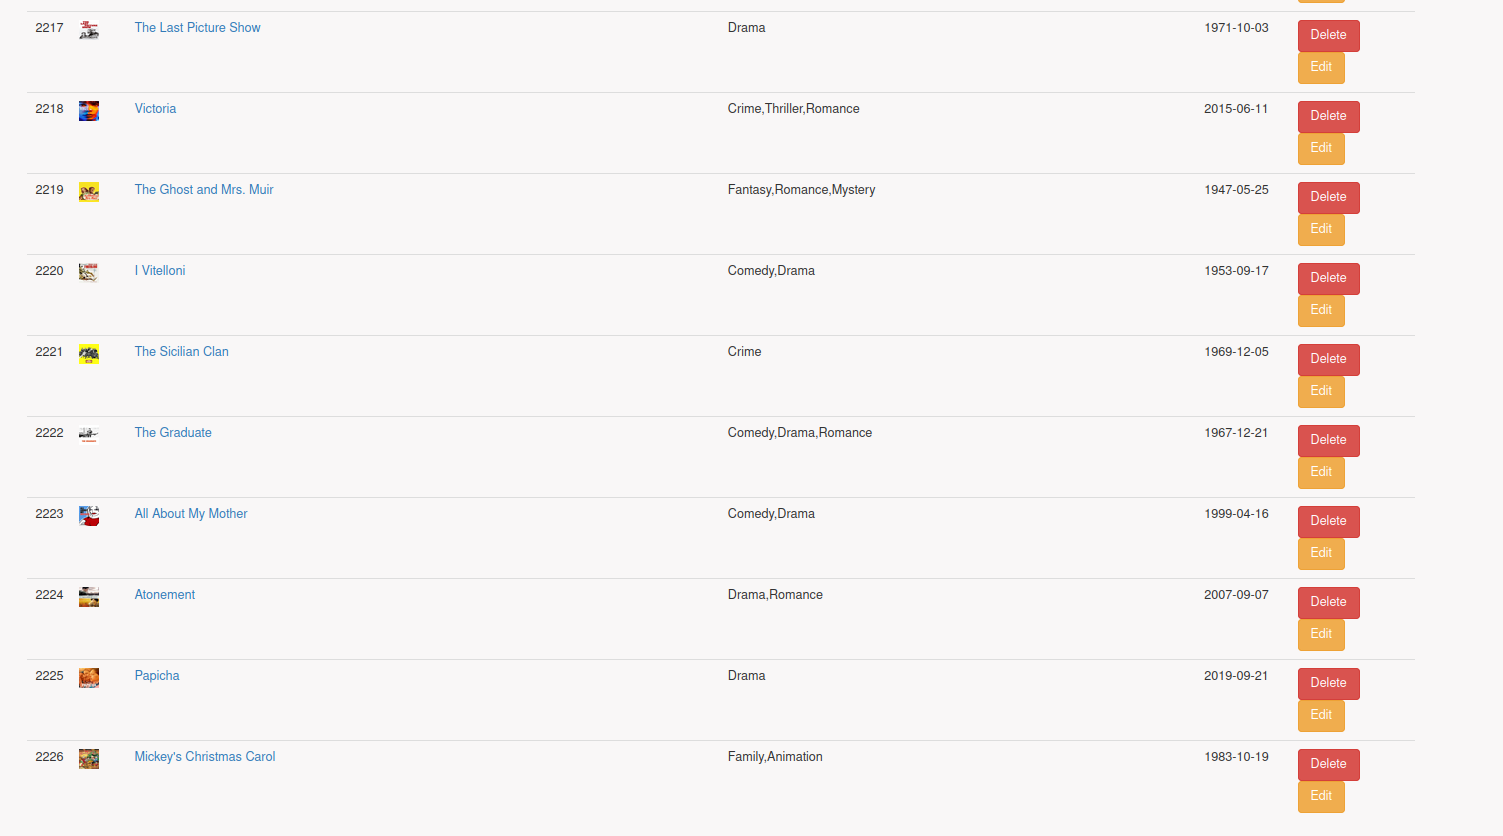
\includegraphics[scale=0.4]{Figs/AdminMovies.png}
        \caption{Hệ thống vẫn đáp ứng thời gian Reponse với hơn 2000 Movies trong Database}
    \end{figure}

    \item Kiểm tra giao diện người dùng: chúng mình đã kiểm tra tính hợp lệ và phản hồi của giao diện người dùng, đảm bảo rằng các chức năng như đăng nhập, đăng ký, thêm phim, đánh giá phim, và tìm kiếm phim đều hoạt động đúng và trở lại kết quả chính xác.

    \item Kiểm tra trạng thái hệ thống: chúng mình đã kiểm tra các trạng thái hệ thống trong các tình huống khác nhau. Ví dụ, chúng mình đã kiểm tra xem hệ thống có xử lý đúng các trạng thái như phim đã được đánh giá hay chưa, người dùng đã đăng nhập hay chưa, và xác định xem các trạng thái này có ảnh hưởng đến chức năng khác hay không.

    \item Kiểm tra tương thích: chúng mình đã kiểm tra tính tương thích của ứng dụng trên các nền tảng và trình duyệt khác nhau. Đảm bảo rằng giao diện người dùng và chức năng hoạt động một cách chính xác trên các nền tảng phổ biến như máy tính, điện thoại di động và máy tính bảng.

    
\end{itemize}
\subsubsection{Kiểm thử hộp trắng (White Box Testing)}
Trong giai đoạn kiểm thử hộp trắng của ứng dụng Spring Movie Review, chúng mình tập trung vào kiểm tra cấu trúc và logic bên trong của hệ thống. Mục tiêu của chúng mình là kiểm tra tính logic và bảo mật của ứng dụng. Dưới đây là một số hoạt động và kỹ thuật chính mà chúng mình đã áp dụng:
\begin{itemize}
    \item Kiểm thử dòng điều khiển: chúng mình đã xác định và kiểm tra các luồng điều khiển trong mã nguồn của ứng dụng để đảm bảo rằng các luồng này hoạt động một cách chính xác và đầy đủ.

    \item Kiểm thử nhánh điều kiện: chúng mình đã kiểm tra các điều kiện trong mã nguồn để đảm bảo rằng tất cả các nhánh điều kiện được xử lý đúng và không có lỗi logic.

    \item Kiểm thử vòng lặp: chúng mình đã kiểm tra các vòng lặp trong mã nguồn để đảm bảo rằng chúng hoạt động chính xác và không gây ra lỗi vòng lặp vô hạn hoặc thiếu sót.

    \item Kiểm thử bảo mật: chúng mình đã xác định và kiểm tra các biện pháp bảo mật được áp dụng trong ứng dụng, bao gồm quản lý quyền truy cập, mã hóa dữ liệu, xác thực và ủy quyền. chúng mình đã đảm bảo rằng hệ thống đáp ứng các tiêu chuẩn bảo mật và bảo vệ quyền riêng tư của người dùng.
\end{itemize}
Bằng cách kết hợp kiểm thử hộp đen và hộp trắng, chúng mình đã đảm bảo rằng ứng dụng Spring Movie Review được kiểm tra một cách toàn diện, từ các khía cạnh bên ngoài đến bên trong. chúng mình đã tìm ra và khắc phục nhiều lỗi và vấn đề tiềm ẩn, đồng thời đảm bảo rằng hệ thống hoạt động đúng, an toàn và có hiệu suất ổn định.

Trên cơ sở kết quả kiểm thử, chúng mình đưa ra các đề xuất và góp ý để nâng cao chất lượng và đáng tin cậy của ứng dụng. Đồng thời, chúng mình cũng đánh giá khả năng của hệ thống trong việc đáp ứng yêu cầu của người dùng và đảm bảo trải nghiệm người dùng tốt nhất.
\subsection{Đánh giá kết quả}
Trong phần này, chúng tôi đánh giá các kết quả thu được từ việc thử nghiệm và phân tích để đánh giá hiệu suất và chất lượng của ứng dụng. Dưới đây là một số kết quả đáng chú ý mà chúng tôi đã nhận thấy:
\begin{itemize}
    \item Tính ổn định: Sau quá trình thử nghiệm, chúng tôi đã xác nhận rằng ứng dụng Spring Movie Review hoạt động ổn định và không gặp phải các lỗi nghiêm trọng hoặc sự cố hệ thống.

    \item Hiệu suất: Chúng tôi đã đo và đánh giá hiệu suất của ứng dụng dựa trên thử nghiệm với tải lượng sử dụng đa dạng. Kết quả cho thấy rằng ứng dụng có thời gian phản hồi nhanh chóng và duy trì hiệu suất ổn định trong các tình huống tải lượng cao.

    \item Bảo mật: Qua quá trình kiểm thử bảo mật, chúng tôi đã xác định và khắc phục các lỗ hổng bảo mật tiềm ẩn trong ứng dụng. Hệ thống đã được cải thiện để đảm bảo an toàn thông tin và bảo vệ quyền riêng tư của người dùng.

    \item Tính năng: Chúng tôi đã kiểm tra các tính năng chính của ứng dụng và xác nhận rằng chúng hoạt động một cách chính xác và đáng tin cậy. Người dùng có thể thực hiện các hoạt động như tìm kiếm, xem chi tiết phim, đánh giá và yêu thích phim một cách dễ dàng và thuận tiện.
    \begin{figure}[H]
        \centering
        \includegraphics*[scale=0.3]{Figs/Evaluate.png}
    \end{figure}
    \item Đáp ứng yêu cầu: Ứng dụng Spring Movie Review đã đáp ứng tốt các yêu cầu và mong đợi của người dùng. Chúng tôi đã nhận được phản hồi tích cực từ người dùng trong việc trải nghiệm và sử dụng ứng dụng.
\end{itemize}
Từ kết quả đánh giá trên, chúng tôi kết luận rằng ứng dụng Spring Movie Review đã đáp ứng thành công mục tiêu và yêu cầu ban đầu. Chúng tôi đã đảm bảo tính ổn định, hiệu suất, bảo mật và tính năng của hệ thống để mang lại trải nghiệm người dùng tốt nhất và đáp ứng nhu cầu của người dùng trong lĩnh vực xem phim.
\section{Kết luận và Hướng phát triển}
\subsection{Ưu điểm của ứng dụng}
\begin{itemize}
    \item Giao diện đẹp và trực quan: Ứng dụng có giao diện người dùng hấp dẫn, dễ sử dụng và trực quan. Người dùng có thể dễ dàng tìm kiếm, xem thông tin và đánh giá các bộ phim.

    \item Hệ thống đánh giá phim: Ứng dụng cung cấp hệ thống đánh giá phim cho phép người dùng đưa ra nhận xét và xếp hạng các bộ phim. Điều này giúp người dùng có cái nhìn tổng quan về chất lượng của một bộ phim trước khi quyết định xem.

    \item Tính năng tìm kiếm và lọc phim: Ứng dụng cung cấp tính năng tìm kiếm và lọc phim dựa trên nhiều tiêu chí như thể loại, năm phát hành, đạo diễn, diễn viên và xếp hạng. Điều này giúp người dùng dễ dàng tìm kiếm và lựa chọn bộ phim phù hợp với sở thích của mình.

    \item Hệ thống xếp hạng và đề xuất phim: Ứng dụng cung cấp hệ thống xếp hạng phim dựa trên đánh giá của người dùng, giúp người dùng tìm kiếm những bộ phim có đánh giá cao từ cộng đồng. Ngoài ra, ứng dụng cũng đề xuất phim dựa trên sở thích của người dùng, mang lại trải nghiệm cá nhân hóa.
\end{itemize}
\subsection{Mặt hạn chế}
\begin{itemize}
    \item Thiếu tính năng tương tác: Hiện tại, ứng dụng chưa tích hợp các tính năng tương tác như chatbot hoặc hệ thống bình luận trực tiếp giữa người dùng. Điều này có thể hạn chế khả năng giao tiếp và chia sẻ ý kiến giữa người dùng.

    \item Hạn chế về thông tin phim: Một số bộ phim có thể thiếu thông tin chi tiết như trailer, diễn viên và nội dung chi tiết. Điều này có thể làm giảm sự hấp dẫn và cung cấp thông tin không đầy đủ cho người dùng.

    \item Thiếu tính năng kết nối xã hội: Ứng dụng chưa tích hợp tính năng kết nối xã hội, như chia sẻ phim yêu thích lên mạng xã hội hoặc mời bạn bè tham gia. Điều này có thể hạn chế khả năng quảng bá và tương tác xã hội của ứng dụng.

    \item Cập nhật dữ liệu chưa đồng bộ: Dữ liệu phim và thông tin liên quan có thể không được cập nhật đồng bộ và thường xuyên. Điều này có thể làm giảm tính chính xác và tin cậy của thông tin trong ứng dụng.
\end{itemize}

Tuy nhiên, những khuyết điểm trên có thể được cải thiện và phát triển trong các phiên bản cập nhật tương lai của ứng dụng.
\subsection{Hướng phát triển}
Hướng phát triển của ứng dụng Spring Movie Review có thể bao gồm:
\begin{itemize}
    \item Phát triển tính năng chatbot: Tích hợp chatbot vào ứng dụng giúp cung cấp hỗ trợ và tương tác tự động với người dùng. Chatbot có thể trả lời câu hỏi, cung cấp gợi ý phim, tư vấn và hỗ trợ người dùng trong quá trình sử dụng ứng dụng.

    
    \item Mở rộng cộng đồng người dùng: Xây dựng một cộng đồng người dùng sôi động trong ứng dụng, cho phép người dùng giao lưu, chia sẻ ý kiến và đánh giá phim. Cung cấp tính năng bình luận, đánh giá và chia sẻ phim để tạo ra môi trường tương tác và thúc đẩy sự tương tác giữa người dùng.

    \item Tích hợp các dịch vụ phim khác: Mở rộng tính năng của ứng dụng bằng cách tích hợp các dịch vụ phim khác, như truyền hình trực tuyến, phim truyện ngắn, hoặc các nền tảng phim nổi tiếng khác. Điều này sẽ mang lại nhiều lựa chọn phim hơn cho người dùng và mở rộng phạm vi sử dụng của ứng dụng.

    \item Tối ưu hóa hiệu năng: Tiếp tục tối ưu hóa hiệu năng của hệ thống để đảm bảo ứng dụng hoạt động mượt mà và đáp ứng tốt với tải lượng người dùng tăng cao. Áp dụng các biện pháp như caching, tối ưu truy vấn cơ sở dữ liệu và phân tán hóa để đảm bảo hiệu suất cao và mở rộng linh hoạt của hệ thống.
\end{itemize}
Từ những hướng phát triển trên, ứng dụng Spring Movie Review có thể ngày càng phát triển và cung cấp trải nghiệm tốt hơn cho người dùng, đồng thời tạo ra một cộng đồng xem phim đa dạng và sôi động.
\subsection{Bài học rút ra}
Trong quá trình thực hiện đồ án Spring Movie Review, chúng ta đã rút ra một số bài học quý giá. Dưới đây là những bài học kinh nghiệm từ việc thực hiện đồ án này:
\begin{itemize}
    \item Sự quan trọng của quản lý thời gian: Quản lý thời gian hiệu quả là yếu tố quan trọng để hoàn thành đồ án theo kế hoạch. Đặt mục tiêu cụ thể và xác định thời hạn cho từng giai đoạn công việc giúp tổ chức công việc một cách có hệ thống và đảm bảo tiến độ đúng.

    \item Kỹ năng tìm kiếm và phân tích thông tin: Trong quá trình thực hiện đồ án, chúng ta đã phải tìm kiếm thông tin từ nhiều nguồn khác nhau và phân tích, lựa chọn những thông tin phù hợp. Kỹ năng tìm kiếm và phân tích thông tin là rất quan trọng để có được kiến thức và công nghệ phù hợp cho dự án.

    \item Hiểu về quy trình phát triển phần mềm: Đồ án Spring Movie Review đã giúp chúng ta hiểu rõ quy trình phát triển phần mềm, từ việc phân tích yêu cầu, thiết kế, triển khai và kiểm thử. Đây là kiến thức quan trọng để thực hiện các dự án phần mềm trong tương lai.

    \item Sự quan trọng của kiến thức về Spring Boot và PostgreSQL: Đồ án này đã cho chúng ta cơ hội nghiên cứu và thực hành với Spring Boot và hệ quản trị CSDL PostgreSQL. Hiểu biết về các công nghệ này rất hữu ích trong việc phát triển ứng dụng web và làm việc với cơ sở dữ liệu.

    \item Kỹ năng làm việc nhóm: Đồ án Spring Movie Review đã yêu cầu chúng ta làm việc nhóm để phân chia công việc và hoàn thành dự án. Kỹ năng làm việc nhóm, giao tiếp và phối hợp là rất quan trọng để đạt được mục tiêu chung và đảm bảo sự thành công của dự án.
\end{itemize}
Tổng kết lại, đồ án Spring Movie Review không chỉ mang lại cho chúng ta kiến thức về phát triển phần mềm và công nghệ, mà còn giúp chúng ta nắm vững các kỹ năng quản lý thời gian, tìm kiếm và phân tích thông tin, làm việc nhóm và hiểu rõ quy trình phát triển phần mềm. Những bài học này sẽ giúp chúng ta trở thành những nhà phát triển phần mềm tài năng và thành công trong tương lai.
\section{Phân chia công việc}
\begin{table}[H]
    \centering
    \caption{Bảng phân chia công việc Nhóm 10 - Spring Movie Review}
    \begin{tabular}{|c|c|c|}
      \hline
      \textbf{STT} & \textbf{Thành viên} & \textbf{Công việc} \\
      \hline
      1 & Nguyễn Hoàng Tân & Thiết kế cơ sở dữ liệu, Thuật toán Recommend, \\
      & & Tạo Pagination, Chức năng tìm kiếm, \\
      & & Call TMDB API, Viết báo cáo, Vẽ Diagram \\
      \hline
      2 & Đỗ Trần Mai Anh & Trang chủ, Trang thông tin phim , Trang Admin \\
      & & Slide, Viết báo cáo \\
      \hline
      3 & Nguyễn Thị Quỳnh Hương & Thanh Navbar, Logo, Tính năng tìm kiếm \\
      & & Viết cáo báo \\
      \hline

    \end{tabular}
  \end{table}
  \begin{center}
  \href{https://github.com/Dev-Aligator/Spring-Movie-Review}{Source code - Spring Movie Review}
  \end{center}
\end{document}
